\chapter{Constructions}\label{chap:constructions}

\begin{epigraph}{14em}{Hermann Weyl}
  The introduction of numbers as \\
  coordinates is an act of violence.
\end{epigraph}

\section{Milnor Spheres}\label{sec:milnor-spheres}
\cite{milnor1956manifolds}

\subsection{The Gromoll-Meyer Sphere}\label{sec:gromoll-meyer}
\cite{gromollmeyer1974curvature}

\section{Plumbing}\label{sec:plumbing}

We now turn our attention to a powerful constructive technique in surgery theory 


\subsection{Intersections in Differential Topology}\label{sec:differential-topology-intersections}

\begin{theorem}[Preimage Theorem]\label{thm:preimage}
	If $f : N \to X$ is a smooth map transverse to a submanifold $M\subset X$ then $S=f^{-1}(M)\subset N$ is a submanifold with the same codimension in $N$ as $M$ in $X$.
\end{theorem}
\begin{proof}
	See the proof of Theorem~6.30 in \cite{lee2013smooth}.
\end{proof}

\begin{remark}\label{rmk:symmetric-preimage-theorem}
	We can get a symmetric version of this theorem as a straightforward corollary. If we have two transverse maps $f : N\to X$ and $g : M\to X$, then the map $f\times g : N\times M \to X\times X$ is transverse to the diagonal submanifold $\Delta\subset X\times X$. \cref{thm:preimage} will then imply that
	\[
		(f\times g)^{-1}(\Delta) \subset M\times N
	\]
	is a submanifold. When $g$ is an embedding, $(f\times g)^{-1}(\Delta)$ can be projected down onto $M$ to get the preimage $f^{-1}(M)$.
\end{remark}

If the manifolds involved in \cref{thm:preimage} are orientable, this preimage $S$ admits a canonical orientation by the following procedure. First of all, recall that for any embedded manifold $M\subset X$ there is an exact sequence of vector bundles by quotienting
\begin{equation}\label{eq:oriented-intersection-number-1}
	\begin{tikzcd}
		0 & {\T M} & {\T X} & {\T X/M} & 0
		\arrow[from=1-1, to=1-2]
		\arrow[from=1-2, to=1-3]
		\arrow[from=1-3, to=1-4]
		\arrow[from=1-4, to=1-5]
	\end{tikzcd}
\end{equation}
where $\T X/M$ is the normal bundle of $M\subset X$. Using the orientations of $X$ and $M$, we can use this exact sequence to get an orientation of the normal bundle $\T X/M$. At every point $p\in S$ of the preimage, the differential map $df$ connects the sequence \cref{eq:oriented-intersection-number-1} to the normal bundle sequence for the embedding $S\subset N$.
\begin{equation}\label{eq:oriented-intersection-number-2}
	\begin{tikzcd}
		0 & {\T_pS} & {\T_p N} & {\T_p N/S} & 0 \\
		0 & {\T_{f(p)}M} & {\T_{f(p)}X} & {\T_{f(p)}X/M} & 0
		\arrow[from=1-1, to=1-2]
		\arrow[from=1-2, to=1-3]
		\arrow["{df_p}", from=1-2, to=2-2]
		\arrow[from=1-3, to=1-4]
		\arrow["{df_p}", from=1-3, to=2-3]
		\arrow[from=1-4, to=1-5]
		\arrow["{df_p}", from=1-4, to=2-4]
		\arrow[from=2-1, to=2-2]
		\arrow[from=2-2, to=2-3]
		\arrow[from=2-3, to=2-4]
		\arrow[from=2-4, to=2-5]
	\end{tikzcd}
\end{equation}
In this diagram \cref{eq:oriented-intersection-number-2}, the rightmost vertical map is an isomorphism by the transversality of $f$ and $M$. This means that we can pullback the orientation on $\T_{f(p)} X/M$ to $\T_p N/S$. Since $\T_p N$ is oriented, the usual ``2-out-of-3'' rule applied to the top row of \cref{eq:oriented-intersection-number-2} gives an orientation of $\T_p S$. See \cref{fig:preimage-orientation} for an example of this orienting procedure.

\begin{figure}[ht]
	\centering
	\import{diagrams}{preimage-orientation.pdf_tex}
	\medskip
	\caption{Orienting a preimage (assuming a clockwise orientation on $X$ and $N$).}\label{fig:preimage-orientation}
\end{figure}

When $M$ and $N$ have complementary dimensions, the preimage $S=f^{-1}(N)\subset M$ is a compact oriented $0$-dimensional manifold. For each point $p\in S$, we have $\T_p S=0$ so the map $\T_p N\to \T_p N/S$ in \cref{eq:oriented-intersection-number-2} is an isomorphism. The orientation of $N$ gives an orientation of $\T_p N$, and the preimage orientation procedure gives us an orientation of $\T_p N/S$. Now we can define:

\begin{definition}
	The \defn{local (oriented) intersection number}[oriented intersection number (local)] of $f$ and $M$ at $p\in S$ is
	\[
		\#_p^X(f, M) = \begin{cases}
			+1 & \T_p N/S \textrm{ has the same orientation as } \T_p N,     \\
			-1 & \T_p N/S \textrm{ has the opposite orientation to } \T_p N.
		\end{cases}
	\]
\end{definition}
Summing over all of the local intersection numbers gives a global quantity.
\begin{definition}
	The \defn{(oriented) intersection number}[oriented intersection number] of a smooth map $f : N \to X$ intersecting a submanifold $M\subset X$ transversally is
	\[
		\#^X(f, M) = \sum_{p\in S} \#_p^X(f, M) \in \Z.
	\]
\end{definition}

\begin{remark}\label{rmk:symmetric-intersection-number}
	For a more symmetric version of this definition when two smooth maps $f : N \to X$ and $g : M \to X$ intersect transversally, we could take inspiration from \cref{rmk:symmetric-preimage-theorem} and define the oriented intersection number of the smooth maps $f$ and $g$ as
	\[
		\#^X(f,g) = \#^{X\times X}(f\times g, \Delta).
	\]
	This symmetric intersection number is graded commutative in the dimensions of $M$ and $N$, i.e.
	\begin{equation}\label{eq:intersection-number-graded-commutative}
		\#^X(f,g) = (-1)^{\dim M\cdot \dim N} \#^X(g,f)
	\end{equation}
\end{remark}

Just as the property of transversality is stable -- resilient to homotopic perturbations -- so too is the oriented intersection number. This follows as a corollary to a more general theorem.

\begin{theorem}
	If $W$ is a compact oriented manifold with boundary, and $H : W \to X$ is a smooth map, then $\#^X(\partial H, M)=0$. Here, we use the notation $\partial H : \partial W \to X$ to refer to the restriction of $H$ to the boundary of $W$.
\end{theorem}

\begin{corollary}
	If $H : [0,1]\times N \to X$ is a smooth homotopy, then $\#^X(H_0, M) = \#^X(H_1, M)$.
\end{corollary}

Applying the construction of the symmetric oriented intersection number gives a map
\begin{equation}\label{eq:oriented-intersection-number-homotopy}
	\lkxfunc{\#^X}{[N,X]\times [M,X]}{\Z}{f,g}{\#^X(f,g)}
\end{equation}
This is a geometric precursor to the intersection form of a manifold, a central object of study in geometric topology.

\begin{remark}
	If we don't assume orientations, we can still get a homotopy invariant intersection number, however we must reduce mod $2$. In this case, we could simply define 
	\[
		\#_2^X(f,M) = |S|\mod 2.
	\]
	This is called the \defn{unoriented intersection number}.
	\todo{elaborate}
\end{remark}

Finally, we'll state a useful result in computer self-intersection numbers -- a way to compute the intersection number of a submanifold with itself.

\begin{theorem}\label{thm:euler-number-self-intersection}
	If $M$ is a closed $m$-dimensional submanifold of a $2m$-dimensional submanifold $X$ then we have
	\[
		\#^X(M, M) = \chi(\T X/M)
	\]
	where $\chi(\T X/M)$ is the Euler number of the normal bundle of $M$.
\end{theorem}
\begin{proof}
	\todo{todo}
\end{proof}

\begin{corollary}\label{thm:euler-number-self-intersection-corollary}
	The Euler number $\chi(\xi)$ of an oriented real vector bundle $\xi : E \to B$ over a compact oriented manifold can be expressed as the intersection number
	\[
		\#^E(z,z) = \chi(\xi)
	\]
	where $z : B \to E$ is the zero section.
\end{corollary}

\todo{add 1.C from \cite{levine1985lectures}}

\subsection{Creating an Intersection Form}

Now let's say that we wanted to construct a $2m$-dimensional manifold with a given intersection form -- specified by a bilinear form $Q$ on the unit lattice $\Z^\ell$ with basis vectors $e_1,\ldots, e_\ell$. Let's call this hypothetical construction $W^{2m}$. Our construction here will allow $W$ to have a boundary, since constructing closed manifolds with a given intersection form is generally harder.
Such a construction would be a partial inverse to \cref{eq:monoid-homomorphism-intersection-form} and allow us to algebraically construct smooth manifolds with complex topology in an easy to understand way.

The simplest possible case is when the lattice is $1$-dimensional, with intersection form
\[
	Q =  (Q_{11})
\]
determined by the single integer $Q_{11}=Q(e_1,e_1)\in \Z$.
The resulting $2m$-manifold $W$ should have middle dimensional homology $\H_m(W)$ free of rank $1$, generated by a cycle $\alpha$ which has self-intersection number $\alpha\tnsv \alpha = Q_{11}$. To construct such a manifold, we start with a $m$-dimensional sphere $S^m$. This will be the submanifold representing the generating cycle $\alpha\in \H_m(W)$. To get a $2m$-dimensional manifold, we ``thicken'' the sphere by choosing a rank $m$ disk bundle $\xi : E \to S^m$ with Euler number $Q_{11}$ (if such a bundle exists). Note that this is equivalent to choosing a vector bundle, since we can move freely between vector and disk bundles by an associated bundle construction. We can now define $W$ as the total space $E$ of the disk bundle. This will be the base case for plumbing constructions.
\begin{figure}[ht]
	\centering
	\import{diagrams}{thickening-sphere.pdf_tex}
	\caption{Two different ``thickenings'' of $S^1$ by $D^1$ bundles.}\label{fig:thickening-sphere}
\end{figure}

Although plumbing non-orientable bundles is certainly possible and interesting in its own right, to keep the resulting manifolds orientable we'll require orientable bundles $\xi$ (this rules out the M\"obius bundle thickening in \cref{fig:thickening-sphere}). With this requirement, $W$ gets a manifold orientation from the orientation of the bundle.
Since disks are contractible, there is a deformation retraction $W\simeq S^m$, and this implies that the middle dimensional homology $\H_m(X)$ is generated by $\iota_*[S^m]$. By \cref{thm:euler-number-self-intersection-corollary}, the self intersection number of $\iota_*[S^m]$ is exactly the Euler number $\chi(\xi)$ which we set to be $Q_{11}$ by our choice of bundle $\xi$.

Vector bundles with a given Euler number don't always exist over an $m$-sphere. For instance, if $m$ is odd, then the Euler number of any bundle over $S^m$ is zero and so $Q_{11}$ must be zero in this case. This isn't a failure of the construction but rather reflects that the intersectio form $Q$ is skew-symmetric when $m$ is odd and so must have zeroes along the diagonal. When $m$ is even however, there are plenty of bundles which have a non-zero Euler number. For instance, the tangent bundle $\T S^m$ has Euler number $2$. This lets us construct a $4k$-manifold with boundary that has intersection form $Q = (2)$. More generally, only even numbers can be achieved as Euler numbers of vector bundles over even-dimensional spheres. This is proved in \cref{cor:expressible-euler-numbers-spheres}.

\subsection{Milnor Manifolds}

\todo{The first constructions of exotic spheres in \cite{milnor1956manifolds} were as boundaries of an $4$-dimensional disk bundles over $S^4$. 
Constructing homotopy spheres in this way shouldn't be too surprising, since some ordinary spheres are formed in this way. For instance, the Hopf fibrations
\[
	\begin{aligned}
		S^0 \lkxto S^1 \lkxto S^1, \\
		S^1 \lkxto S^3 \lkxto S^2, \\
		S^3 \lkxto S^7 \lkxto S^4, \\
	\end{aligned}
\]
express the spheres $S^{2k-1}$ as total spaces of an $S^{k-1}$ bundle over $S^k$ for $k\in\{1,2,4\}$. Equivalently, the spheres $S^{2k-1}$ can be thought of as boundaries of the total spaces of $D^k$ bundles over $S^k$.}

\subsection{Plumbing Multiple Bundles}

Let's now consider the case of a $2$-dimensional lattice, and try to construct a manifold with intersection form $Q$ given by the $2\times 2$ integer matrix:
\[
	Q = \begin{pmatrix} Q_{11} & Q_{12} \\ Q_{21} & Q_{22}\end{pmatrix}.
\]
This matrix should be symmetric when $m$ is even and skew-symmetric when $m$ is odd. To begin constructing a manifold, we want $\H_m(W)$ to be free of rank $2$, generated by cycles $\alpha$ and $\beta$ with intersection numbers specified by the matrix $Q$. The simplest case is when $|Q_{12}|=|Q_{21}|=0$, i.e. the intersection forms is represented by a diagonal matrix and splits as a direct sum $Q=Q_1\oplus Q_2$. In this case, by \cref{prop:connected-sum-intersection-form}, we can define
\[
	P(Q_1\oplus Q_2) = P(Q_1)\+ P(Q_2).
\]
In fact, this construction lets us realize any diagonal matrix as the intersection form of a manifold, assuming all entries along the diagonal are the Euler numbers of some oriented bundle (even if $m$ is even and zero if $m$ is odd).

The next simplest case is when $|Q_{12}|=|Q_{21}|=1$. In this case, we'd want $\H_m(W)$ to be free of rank $2$, generated by cycles $\alpha$ and $\beta$ which intersect only once. The natural thing to do would be to start with a wedge of two $m$-spheres $S^m_1\vee S^m_2$. This should be the homotopy type of the constructed manifold $W$. Next, we need to ``thicken'' this space into a $2m$-manifold by rank $m$ disk bundles $\xi_i : D(E_i) \to S^m_i$ for $i\in\{1,2\}$. However, the total spaces of these bundles still need to be glued together so as to form a manifold. This glueing can be done in a ``criss-cross'' manner. If $S^m_1$ and $S^m_2$ are wedged together at points $x_1$ and $x_2$, we begin by choosing disks $D_i^m\subset S^m_i$ which are neighborhoods of these points. The bundles $\xi_i$ then admit local trivializations, so we get neighborhoods $D_i^m\times D^m_i \subset D(E_i)$ of the points $x_i$ in the total space of the bundle. Finally, we choose diffeomorphisms $g : D_1^m \to D_2^m$ and $h : D_1^m \to D_2^m$ which either both preserve orientations or reverse them.

\begin{definition}\label{def:plumbing}
	The \defn{plumbing} of $D(E_1)$ and $D(E_2)$ at the points $x_1$ and $x_2$ is the quotient space $E_1\square E_2 =D(E_1)\cup_f D(E_2)$ where $f$ is the map
	\[
		\lkxfunc{f}{D_1^m\times D_1^m}{D_2^m\times D_2^m}{(x,y)}{(h(y), g(x)).}
	\]
\end{definition}

Note that away from the neighborhoods $D_1^m\subset S^m_1$ and $D_2^m\subset S^m_2$, the plumbed manifold still looks like the total space of a disk bundle. This allows us to plumb together multiple bundles, or plumb together two bundles at multiple points by choosing distinct disk neighborhoods for each point.

\begin{figure}[ht]
	\centering
	\import{diagrams}{plumbing-two-circles-smoothed.pdf_tex}
	\caption{A plumbing of two trivial circle bundles with smoothed corners.}\label{fig:plumbing-two-circles}
\end{figure}

\begin{remark}\label{rmk:smoothing-corners}
	The plumbing has an a priori smooth structure everywhere except at the ``corners'' which arise from the boundaries $\partial D_1^m\times \partial D_1^m \cong \partial D_2^m\times \partial D_2^m$ in $P$. To smooth these out, \todo{write about smoothing out corners}
\end{remark}

Now let's study the intersection theory of the plumbed manifold. It's clear that the submanifolds $S_1^m$ and $S_2^m$ intersect transversally at a single point.

\begin{proposition}
	If $x$ is the intersection point of $S_1^m$ and $S_2^m$, then we have
	\[
		\#^{E_1\square E_2}_{x}(S_1^m, S_2^m) = \begin{cases}
			+1 & h \textrm{ and }g\textrm{ preserve orientations}, \\
			-1 & h \textrm{ and }g\textrm{ reverse orientations}.  \\
		\end{cases}
	\]
\end{proposition}
\begin{proof}
	\todo{cite}
\end{proof}

As a corollary, if we plumb together two bundles at $m$ points with a positive orientation (let's call this manifold $E_1\square^m E_2$), then the intersection number is \[\#^{E_1\square^m E_2}(S^m_1, S^m_2)=m.\] The same thing with $m$ points and a negative orientation gives the intersection number \[\#^{E_1\square^{-m} E_2}(S^m_1,S^m_2)=-m.\]
We have thus have a way to construct a $4k$-manifold $W^{4k}$ and $(4k+2)$-manifold $W^{4k+2}$ with intersection forms
\[
	Q_{W^{4k}} = \begin{pmatrix} 2e_1 & m \\ m & 2e_2\end{pmatrix}
	\quad\textrm{and}\quad
	Q_{W^{4k+2}} = \begin{pmatrix} 0 & m \\ -m & 0\end{pmatrix}
\]
for any $e_1, e_2,m\in \Z$. This approach generalizes to lattices of higher dimensions, and we arrive at a basic theorem regarding plumbing.

\begin{theorem}
	Suppose $Q$ is an even $m$-symmetric bilinear form on an $\ell$-dimensional lattice $\Lambda$ given by an $\ell\times \ell$ integer matrix. Then there exists a $2m$-dimensional manifold $P(Q)$ with isomorphism $\H_{m}(P(Q))\cong \Lambda$ under which the intersection form of $P(Q)$ is exactly the bilinear form $Q$.
\end{theorem}

\begin{proof}
	Hello world


	\begin{lemma}
		For each integer $q\geq 1$, there is a homotopy equivalence
		\[
			S^m\vee_q S^m \simeq S^m\vee S^m \vee \bigvee_{q-1} S^1,
		\]
		where $S^m\vee_q S^m$ denotes the wedge sum of two $m$-spheres at $q$ points.
	\end{lemma}
	\begin{proof}
		\todo{finish}
	\end{proof}

	\todo{finish}
\end{proof}

\subsection{Plumbing Along a Tree}

While plumbing from a matrix is a nice general way to build a manifold with a given intersection form, many examples we consider in this thesis arise from a tree.

\begin{definition}
	A \defn{tree} $T$ is a finite connected contractible $1$-dimensional simplicial complex, i.e. a finite connected graph with no cycles. An \defn{weighted tree}[tree (weighted)] is a pair $(T,w)$ consisting of a tree $T$ and a map $w : \Vert(T) \to \Z$ assigning a \defn{weight} $w(v)\in \Z$ to each vertex $v$ of the tree.
\end{definition}

Given a tree $T$ with vertices $\{e_1,\ldots, e_\ell\}$ and integral weights $w$, consider the $m$-symmetric matrix given by
\[
	Q_{ij} = \begin{cases}
		w(e_i)    & i=j,                       \\
		(\pm 1)^m & (i,j)\in \textrm{Edge}(T), \\
		0         & \textrm{otherwise}.
	\end{cases}
\]
In the skew-symmetric case, we'll adopt the convention that the upper-triangular part of the matrix is positive. Many of the matrices we're interested arise from trees in this way. For instance, the $E_8$ matrix defined in terms of the $E_8$ lattice in \cref{def:E8-lattice} arises from the Dynkin diagram for the exceptional Lie group $\E_8$.
\begin{proposition}
	The ${E_8}$ bilinear form is associated to the tree
	\[
		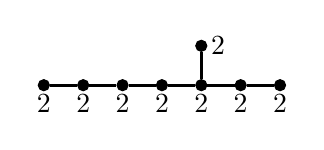
\begin{tikzpicture}
			\tikzset{dynode/.style={circle, draw, fill=black,
						minimum size=4pt, inner sep=0pt}}
			\tikzset{dyline/.style={line width=1pt}}
			\tikzset{dydash/.style={line width=1pt, dashed}}

			\begin{scope}[yshift=-10em, xshift=0]
				\node[dynode] (a1) at (0,0) {};
				\node[dynode] (a2) at (0.5,0) {};
				\node[dynode] (a3) at (1,0) {};
				\node[dynode] (a4) at (1.5,0) {};
				\node[dynode] (a5) at (2,0) {};
				\node[dynode] (a6) at (2.5,0) {};
				\node[dynode] (a7) at (3,0) {};
				\node[dynode] (a8) at (2,0.5) {};

				\draw[dyline] (a1) -- (a2) -- (a3) -- (a4) -- (a5) -- (a6) -- (a7);
				\draw[dyline] (a5) -- (a8);

				\node[below] () at (a1) {$2$};
				\node[below] () at (a2) {$2$};
				\node[below] () at (a3) {$2$};
				\node[below] () at (a4) {$2$};
				\node[below] () at (a5) {$2$};
				\node[below] () at (a6) {$2$};
				\node[below] () at (a7) {$2$};
				\node[right] () at (a8) {$2$};
			\end{scope}
		\end{tikzpicture}
		\quad\implies\quad
		\begin{pmatrix}
			2 & 1 &   &   &   &   &   &   \\
			1 & 2 & 1 &   &   &   &   &   \\
			  & 1 & 2 & 1 &   &   &   &   \\
			  &   & 1 & 2 & 1 &   &   &   \\
			  &   &   & 1 & 2 & 1 & 0 & 1 \\
			  &   &   &   & 1 & 2 & 1 & 0 \\
			  &   &   &   & 0 & 1 & 2 & 0 \\
			  &   &   &   & 1 & 0 & 0 & 2 \\
		\end{pmatrix}
	\]
	where each vertex of the tree is weighed by $2$.
\end{proposition}

It's interesting to note that if $Q$ is a matrix associated to a tree $T$, then $P(Q)$ has a $1$-skeleton homotopy equivalent to $T$. This connection between the $1$-skeleton and plumbing along a tree or graph was first noticed by Hirzebruch. It makes sense then why we'd care about matrices arising from trees instead of from general graphs which may contain cycles -- cycles break the simple-connectedness of the constructed manifold and are thereby much more complicated to work with.

\section{Knots and Branched Coverings}\label{sec:brieskorn}
\cite{milnor1968hypersurfaces}
\cite{kauffman1987knots}
